\problemname{Proteins}

\illustration{.3}{protein}{Protein molecule by \href{http://commons.wikimedia.org/wiki/File:Porin.qutemol.ao.png}{ALoopingIcon}}

Magnus is a biologist. He is playing with proteins all day long and now he wants to know what these
molecules look like. He has heard that X-ray crystallography can be used to get images of proteins that contain a lot of sulfur atoms. Magnus does not think his proteins contain enough sulfur,
but he is willing to change them to get this to work. Magnus has bacteria producing his proteins for
him, and he is planning to mutate these bacteria to change the proteins.

Magnus knows the DNA strings coding his proteins and how the DNA is translated into the amino-acid
sequence making up the protein. The first three letters in the code determine the first amino acid,
the following three letters determine the second, and so on. Whenever those three letters are ATG
(in that order) the amino acid methionine will be incorporated into the protein. Methionine contains
a sulfur atom, so Magnus wants to have many methionines in his proteins. Magnus can only change the DNA code by inserting letters. This, however, takes
a lot of time for each letter he wants to insert. Knowing that you are good at computer stuff, he
asks you for help. Can you figure out the smallest number of letters that need to be inserted into
the DNA code to make it code for $n$ methionines?

For example, the DNA string TGATGC codes for no methionines, but adding an A in the beginning turns
it into ATGATGC which has two ATG blocks and thus codes for two methionines. This is the first
sample input and a solution to the second sample input is shown in the figure below.

\begin{figure}[h]
  \centering
  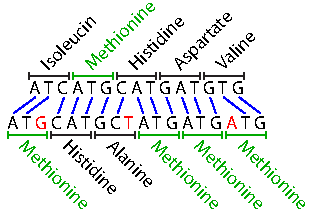
\includegraphics[width=0.5\textwidth]{example}
\end{figure}

\section*{Input}
The first line of input contains a single positive integer $n\leq10^6$, the number of methionines to
be included in the protein. The second line contains a non-empty DNA string of at most $1000$
letters, each either A, T, G, or C.

\section*{Output}
Output a single integer, the smallest number of letters that can be inserted into the DNA string to
make at least $n$ of its three-letter blocks be ATG.
